\section{Project 2}
A simple and easy BAD algorithm to implement in software, since there are limited hardware resources
in a mobile phone, is the \emph{recursive averaging} which calculates the average power level for a
block of fragments from a discretized analog signal. The blocks should large enough to get calculate
an interval but small enough to quickly respond to changes in power amplitude. 
The advanced algorithm is based upon the on the same, \emph{recursive averaging}, algorithm.
In addition, a filter is added to remove the noise which should have even less impact on the BAD. 

Three various baby and noise sounds were provided. The sample frequency for all of the recorded 
files are 8 kHz. In Figure \ref{fig:baby_spec} and Figure \ref{fig:noise_spec} the power/frequency 
spectrum is plotted for baby respective noise sounds. Because the power level is unporportionally 
low for some baby sound recordings an enhanced plot is displayed in Figure~\ref{fig:enhanced}. 
From the plots it can be seen that the baby sound spectrum is between $\sim$ 300-2500 Hz and the 
noise sound spectrum is below 200 Hz and between $\sim$1300-2100 Hz. To get the wanted effect from 
the advanced algorithm a bandpass filter with a window between 300-1300 Hz is the optimal solution. 
The noise is filtered but the baby sound are kept.

\begin{figure}[h]
  \centering
  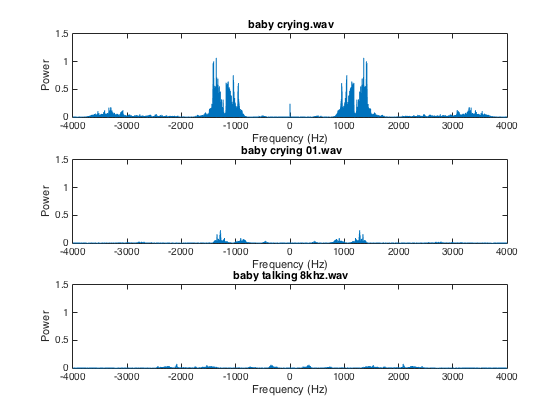
\includegraphics[width=1\textwidth]{sections/freq_spec_baby_linkaxis.png}
  \caption{Bla bla bla}
  \label{fig:baby_spec}
\end{figure}

\begin{figure}[h]
  \centering
  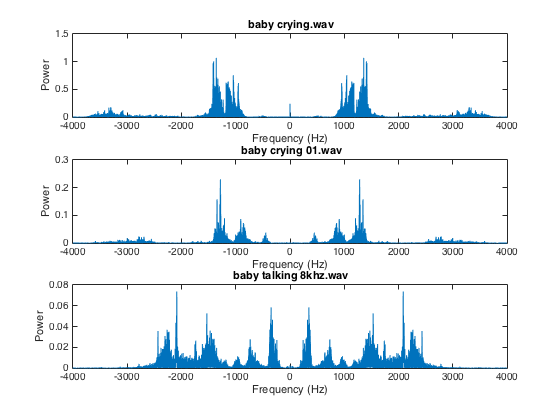
\includegraphics[width=1\textwidth]{sections/freq_spec_babyFix.png}
  \caption{Bla bla bla}
  \label{fig:enhanced}
\end{figure}

%\begin{figure}[!hp]
%  \centering
%  \begin{minipage}[b]{0.4\textwidth}
%    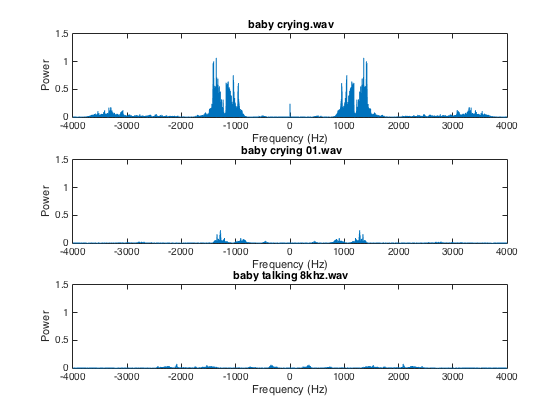
\includegraphics[width=1\textwidth]{sections/freq_spec_baby_linkaxis.png}
%    \caption{Fig111}
%  \end{minipage}
%  \hfill
%  \begin{minipage}[b]{0.4\textwidth}
%    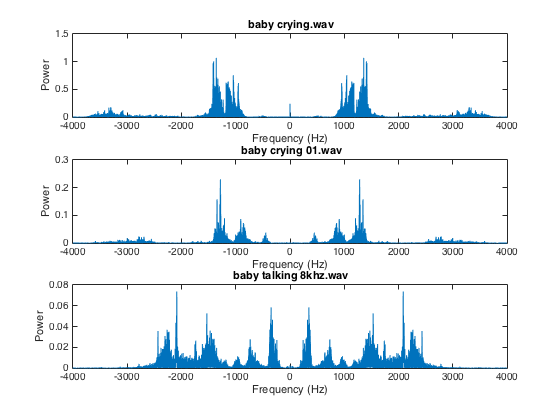
\includegraphics[width=1\textwidth]{sections/freq_spec_babyFix.png}
%    \caption{Fig222}
%  \end{minipage}
%\end{figure}

\begin{figure}
  \centering
  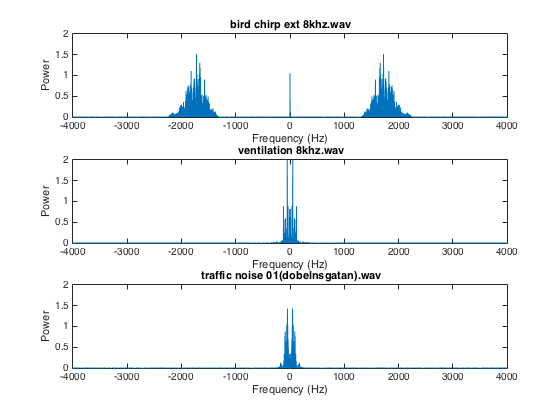
\includegraphics[width=1\textwidth]{sections/freq_spec_noise_linkaxis.png}
  \caption{Bla bla bla}
  \label{fig:noise_spec}
\end{figure}
